\documentclass[openany]{article}

\usepackage[utf8]{inputenc}
\usepackage{amsmath}
\usepackage{latexsym}
\usepackage{IEEEtrantools}
\usepackage[dvipsnames]{xcolor}
\usepackage{soul}
\DeclareRobustCommand{\hlred}[1]{{\sethlcolor{BrickRed}\hl{#1}}}

\usepackage{amsmath}
\usepackage{latexsym}
\usepackage{IEEEtrantools}
\numberwithin{equation}{section}
\usepackage{color}
\usepackage{xcolor, soul}
\sethlcolor{yellow}
\usepackage[dvipsnames]{xcolor}
\usepackage{listings}
\usepackage{courier}
\usepackage{array}
\usepackage{calc}

\usepackage{titlesec}
\usepackage{lipsum}
\usepackage{circuitikz}
\usepackage{floatrow}


\lstset{
language=C,                % choose the language of the code
basicstyle=\ttfamily\normalsize,       % the size of the fonts that are used for the code
numbers=left,                   % where to put the line-numbers
numberstyle=\tiny,      % the size of the fonts that are used for the line-numbers
stepnumber=0,                   % the step between two line-numbers. If it is 1 each line will be numbered
numbersep=5pt,                  % how far the line-numbers are from the code
backgroundcolor=\color{white},  % choose the background color. You must add \usepackage{color}
showspaces=false,               % show spaces adding particular underscores
showstringspaces=false,         % underline spaces within strings
showtabs=false,                 % show tabs within strings adding particular underscores
frame=single,           % adds a frame around the code
tabsize=1,
captionpos=b,           % sets the caption-position to bottom
breaklines=true,        % sets automatic line breaking
breakatwhitespace=false,
numberblanklines=false,
escapeinside={\%*}{*)}}


%\usepackage{pgfplots}

\title{Progetto 1.1 “Analisi Comparativa tra OS161 e altri Sistemi Operativi Open-Source all'Avanguardia per Sistemi Embedded e Computer General Purpose”}
\author{S308538 - Gaetano Insinna}
\date{Programmazione di Sistema - a.a. 2023-24}

\usepackage{geometry}
\geometry{a4paper, top=3cm, bottom=3cm, left=2.5cm, right=2.5cm}

\usepackage{courier}
%\renewcommand*\familydefault{\ttdefault} %% Only if the base font of the document is to be typewriter style
\usepackage[T1]{fontenc}

\renewcommand{\contentsname}{Indice} %Change the name of ToC
\renewcommand{\lstlistingname}{Code}% Listing -> Code
\begin{document}

\maketitle
\thispagestyle{empty}
\newpage
\tableofcontents

\section{Memoria Virtuale}
In questo capitolo tratteremo della memoria virtuale: a una breve introduzione teorica seguirà la comparazione tra OS161 e xv6 ovvero il sistema operativo che stiamo analizzando.
\subsection{Introduzione}
La memoria virtuale è una tecnica di gestione della memoria che simula un aumento della memoria principale vista da parte di ogni processo. Questa tecnica introduce diversi vantaggi:
\begin{enumerate}
    \item un processo in esecuzione può essere più grande della memoria fisica, quindi un processo non è limitato dalla quantità di memoria attualmente a disposizione
    \item un processo può essere eseguito anche se non è caricato interamente in memoria principale, quindi possono essere eseguiti più programmi contemporaneamente
    \item i processi possono condividere librerie e files
    \item vengono effettuate un numero minore di operazioni di page swapping in quanto in memoria saranno caricate sole le pagine più utilizzate e non tutte le pagine, anche se attualmente non utilizzate, di un singolo processo
\end{enumerate}
\subsubsection{Implementazione della memoria virtuale}
La tecnica su cui si basa la memoria virtuale è chiamata paging e consiste nel dividere la memoria in porzioni fisse. Esse prendono il nome di:
\begin{itemize}
    \item pagine: porzione della memoria virtuale
    \item frames: porzione della memoria fisica
\end{itemize}
è importante sottolineare, tuttavia, che la dimensioni di una pagina è uguale a quella di un frame e viceversa.

Gli indirizzi prodotti da una CPU sono degli indirizzi virtuali che non corrispondono immediatamente agli indirizzi della memoria fisica, occorre infatti eseguire delle operazioni per trovare questa corrispondenza. Per eseguire ciò viene introdotto il concetto di page table che altro non è che una tabella nella quale vengono salvati gli indirizzi dei frames. Essi poi possono essere ricavati tramite una ricerca per mezzo del pagina.

Esula da questo lavoro scendere nel dettaglio sul funzionamento della page table e sulla comparazione tra le diverse page table esistenti, ma si esprime una introduzione per poter trattare un confronto tra i sistemi operativi OS161 e xv6.

Per capire il funzionamento di una page table e come avviene la traduzione tra indirizzo logico a fisico, l'indirizzo generato dalla CPU viene diviso in due parti che prendono il nome di:
\begin{itemize}
    \item page number: viene utilizzato come indice per accedere alla page table, la entry corrispondente è il frame number
    \item page offset: indica dove si trova il dato richiesto all'interno della pagina e, di conseguenza, all'interno del frame
\end{itemize}
Unendo il frame number, trovato come entry della page table, e il page/frame offeset si ottiene l'indirizzo della memoria fisica.

\subsubsection{Memory Management Unit e Translation Lookaside Buffer}
Il lavoro descritto nelle sezioni precedenti è svolto da un particolare dispositivo hardware chiamato Memory Manangement Unit o MMU. Per eseguire la traduzione degli indirizzi esso utilizza, oltre alla modalità già presentata, una seconda ovvero lavora con un hardware dedicato, implementato con memoria cache, chiamato Translation Lookaside Buffer o TLB. Esso possiede una quantità finita di elementi delle tabella delle pagine e viene utilizzato come vera e propria memoria cache degli indirizzi che vengono tradotti più spesso. Gli elementi del TLB vengono chiamati entries e, grazie ad un accesso diretto, qualora il frame ricercato sia in TLB (TLB Hit) l'indirizzo da tradurre viene generato in maniera molto più veloce, altrimenti accade un TLB Miss e il frame viene calcolato nella maniera descritta sopra.

\hlred{capire se aggiungere o meno Page Fault e TLB Miss - Demand Paging}
\subsection{Memoria Virtuale in OS161}
Il sistema operativo OS161 è basato su un'architettura \lstinline{MIPS} a 32-bit.
La memoria in OS161 è allocata in modo contiguo e misura \lstinline{4 GB}. I primi \lstinline{2 GB} sono riservati alla memoria utente e i secondi sono dedicati alla memoria kernel. Il kernel è mappato in una porzione dello spazio di indirizzamento di ogni processo in modo che esso possa vedere i processi user in maniera semplice. Per poter accadere ciò ci sono dei metodi di protezione attivi per far sì che quando si lavora in modo non privilegiato si possa vedere solamente una parte specifica dell'address space.
Nello specifico la memoria è divisa in 4 porzioni:
\begin{enumerate}
   \item \lstinline{kuseg}: User and supervisor mode; TLB-mapped, cacheable. 
   
   È un segmento di \lstinline{2 GB} che va da \lstinline{0x00000000} a \lstinline{0x7fffffff} e rappresenta la memoria dove risiedono i programmi a livello utente. È mappato in TLB così da poter effettuare la traduzione da indirizzo logico a indirizzo fisico.
    \item \lstinline{kseg0}: Supervisor mode only; direct-mapped, cached.

    È un segmento che va da \lstinline{0x80000000} a \lstinline{0x9fffffff},  rappresenta la memoria kernel quindi non è mappato in TLB per far sì che ci sia una traduzione veloce tra indirizzo logico e indirizzo fisico semplicemente sottraendo all'indirizzo l'indirizzo di base della stessa porzione e ha la cache.
    \item \lstinline{kseg1}: Supervisor mode only; direct-mapped, uncached.

    È un segmento che va da \lstinline{0xa0000000} a \lstinline{0xbfffffff} e rappresenta la memoria dei dispositivi di I/O per questo motivo non è mappato in TLB e non prevede la cache 
    \item \lstinline{kseg2}: Supervisor mode only; TLB-mapped, cacheable.

    È un segmento di memoria che va da \lstinline{0xc0000000} a \lstinline{0xffffffff} ed è inutilizzato 
\end{enumerate}

\begin{figure}[hbt!]
    \centering
    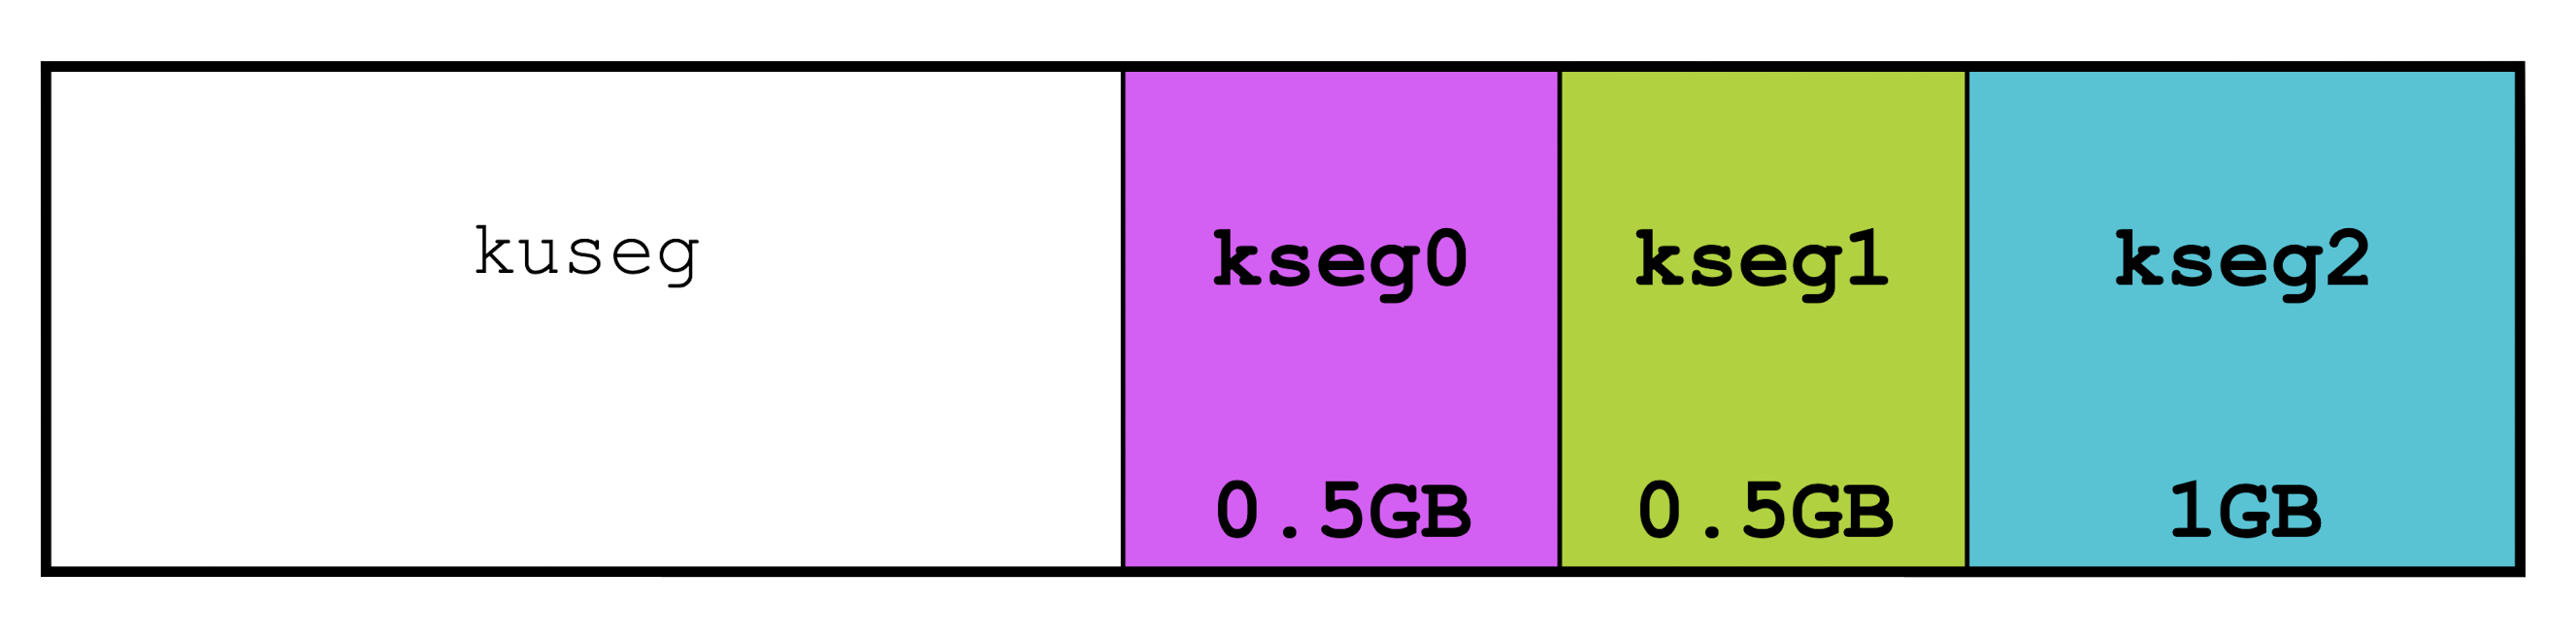
\includegraphics[width=0.7\textwidth]{Memoria Virtuale/images/kernel memory os161.png}
    \caption{Rappresentazione della memoria di OS161}
    \label{kmemos161}
\end{figure}

\subsubsection{Inizializzazione e avvio del kernel}
Il kernel viene avviato tramite la funzione assembler \lstinline{kern/arch/sys161/main/start.S}.
Questa è una panoramica del kernel all'avvio di OS161 in una memoria RAM di \lstinline{1 MB}:
\begin{figure}[hbt!]
    \centering
    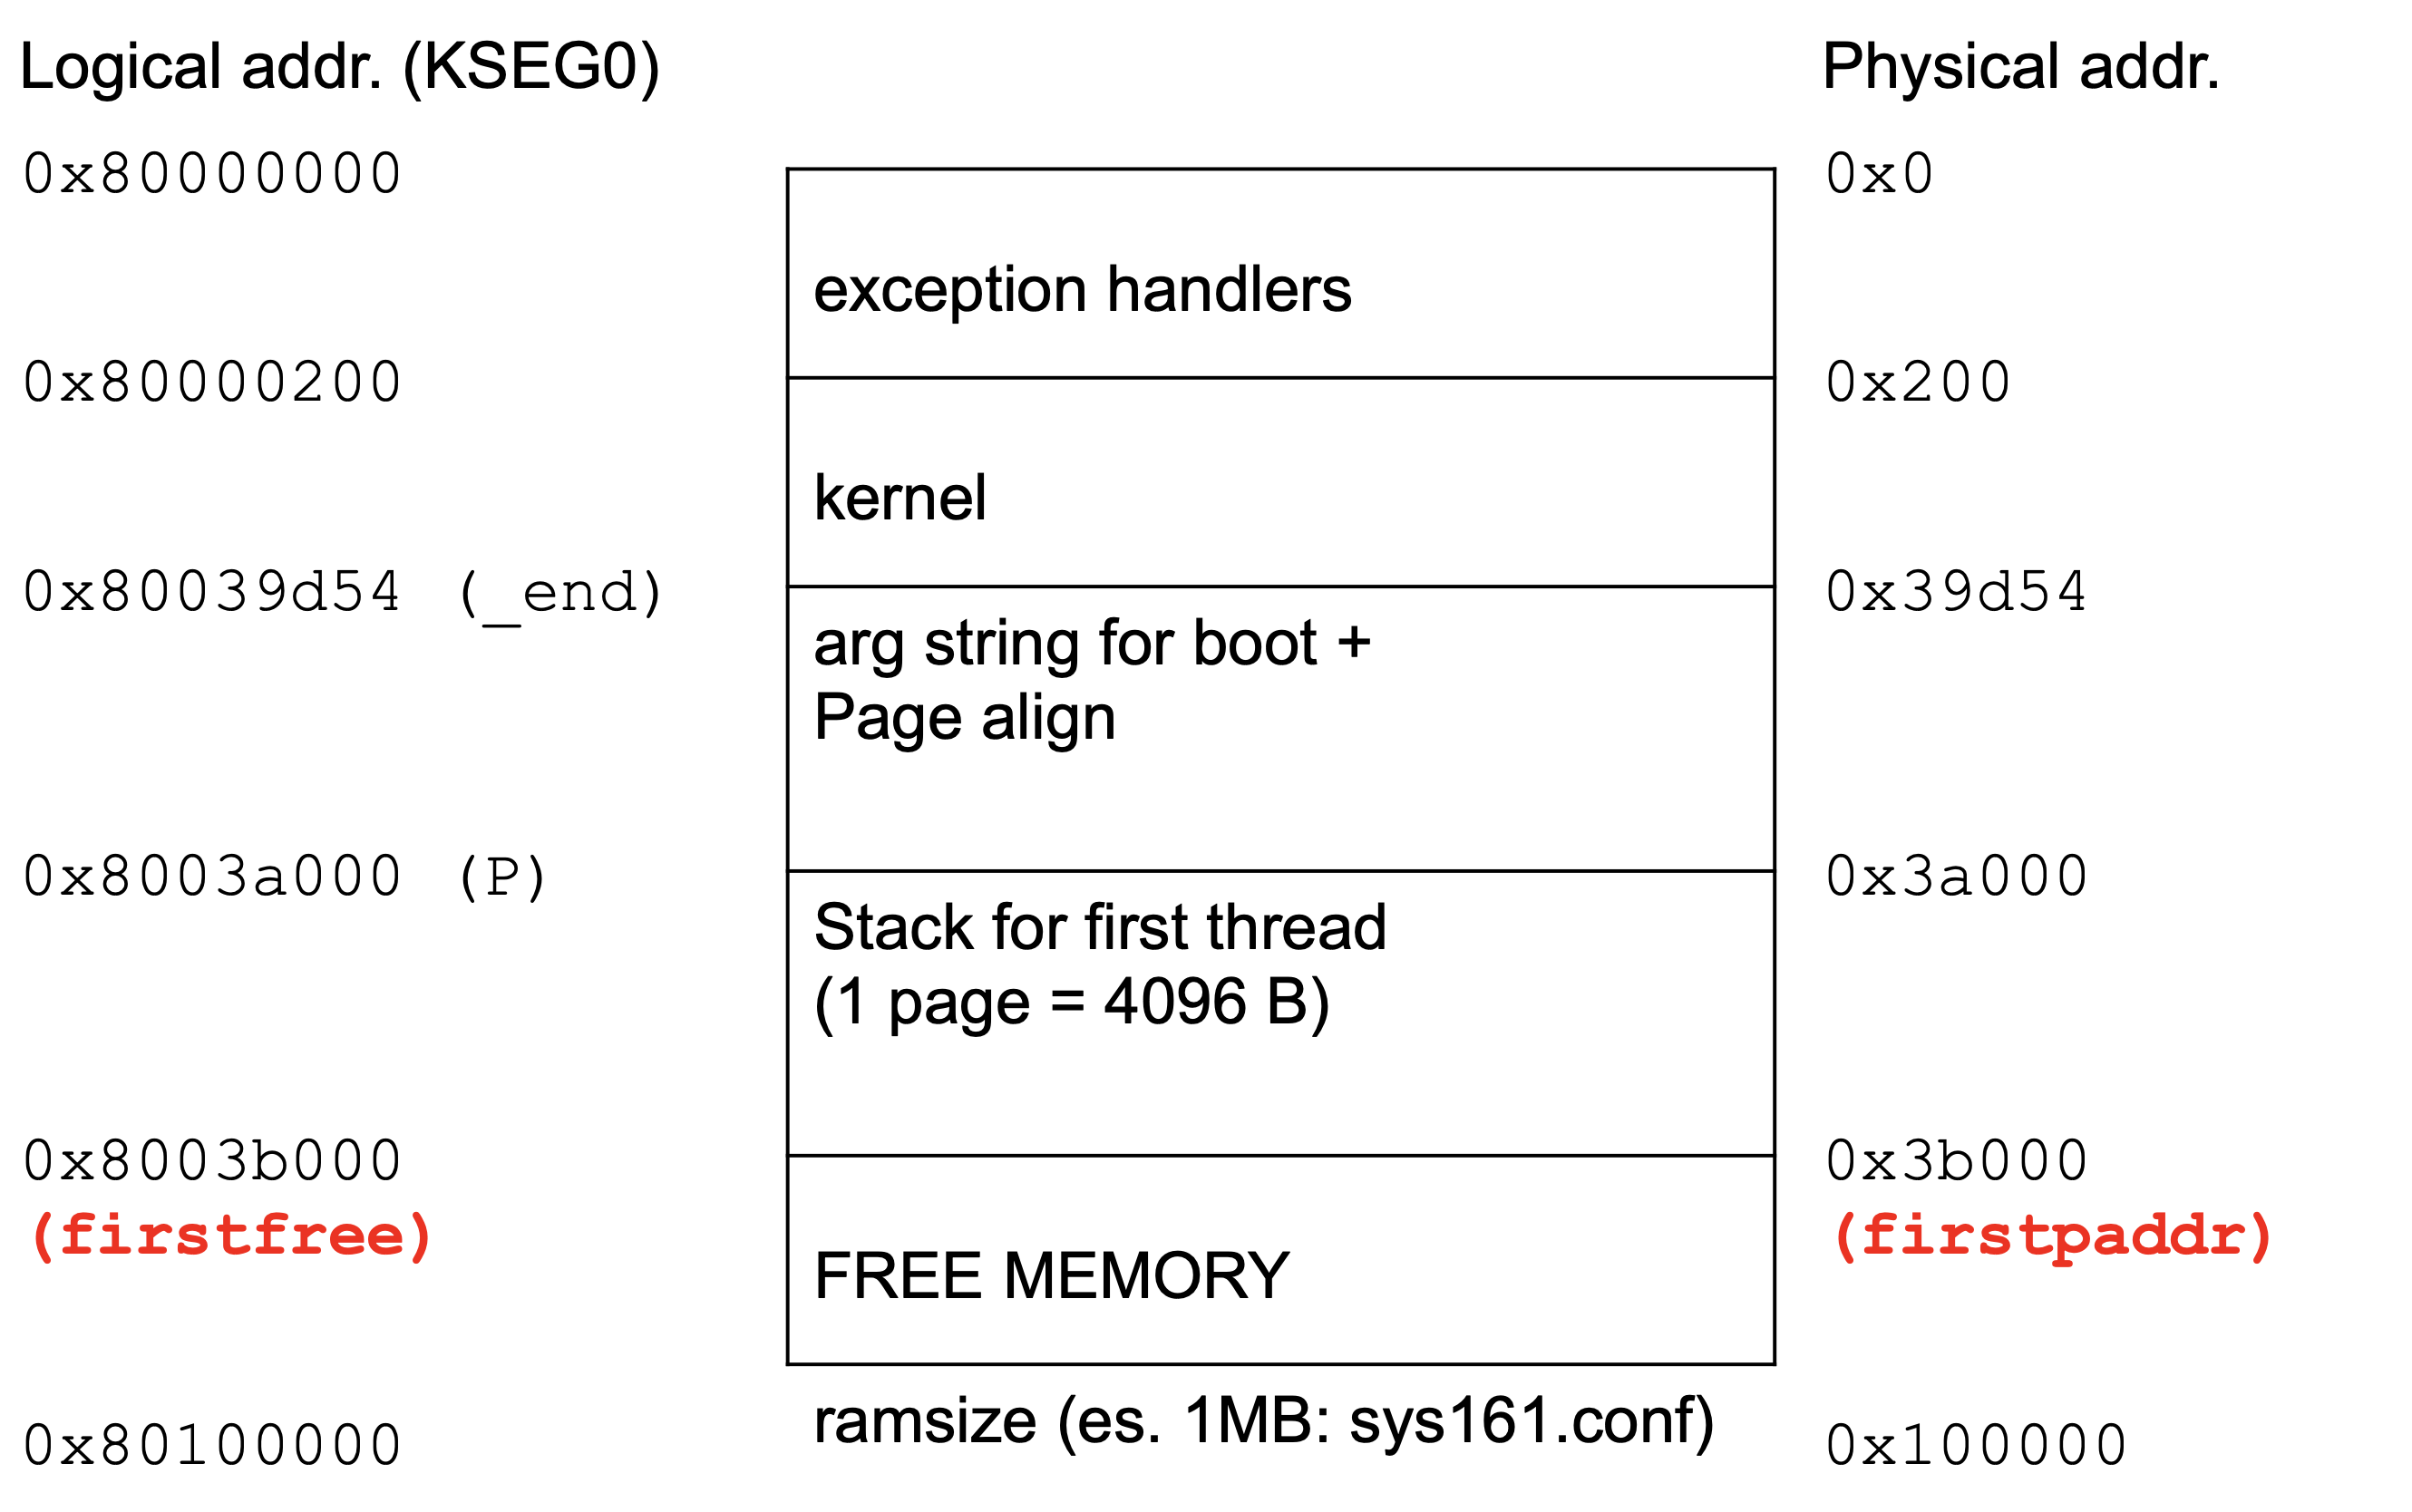
\includegraphics[width=0.7\textwidth]{Memoria Virtuale/images/kernel snapshot.png}
    \caption{Configurazione iniziale del kernel}
    \label{kernel_snapshot}
\end{figure}

Come possiamo vedere quando si fa bootstrap del kernel in RAM si trovano diverse sezioni:
\begin{enumerate}
    \item gestori delle eccezioni
    \item il kernel
    \item stringhe per il boot (anche se nella versione base di OS161 non è richiesta alcuna stringa, ma potrebbe essere inserita) e allineamento di pagine 
    \item lo stack del primo thread di kernel
    \item memoria libera
\end{enumerate}
Questa configurazione può cambiare, il kernel può aumentare se vengono implementate nuove funzioni.

Si può notare che finito il boostrap, vengono salvati gli indirizzi di memoria fisica (\lstinline{firstpaddr}) e logico (\lstinline{firstfree}).


\begin{lstlisting}[caption=Parte del codice di avviamento del kernel]
    /* Gestione dello stack per il primo thread di kernel */
   .frame sp, 24, $0	/* 24-byte sp-relative frame; return addr on stack */
   .mask 0x80000000, -4	/* register 31 (ra) saved at (sp+24)-4 */
   addiu sp, sp, -24
   sw ra, 20(sp)
   la s0, _end		/* stash _end in a saved register */

   /* Gestione della bootstring e allineamento di pagina*/
   move a1, a0		/* move bootstring to the second argument */
   move a0, s0		/* make _end the first argument */
   jal strcpy		/* call strcpy(_end, bootstring) */
   nop			    /* delay slot */
   /. . ./
   sw t0, firstfree	/* remember the first free page for later */
   /. . ./
   
   /* Gestione delle eccezioni */
   li a0, EXADDR_UTLB
   la a1, mips_utlb_handler
   la a2, mips_utlb_end
   sub a2, a2, a1
   jal memmove
   nop
   /. . ./
   
   /* Inizializzazione della TLB */
   jal tlb_reset
   nop
   /. . ./
   
   /* Chiamata del kernel */
   jal kmain
   move a0, s0			/* in delay slot */
   /. . ./
\end{lstlisting}

\subsubsection{Allocazione}
L'allocazione della memoria, di default, è gestita da un allocatore che prende il nome di \lstinline{dumbvm} che prevede solamente le operazioni di base. Le allocazioni di memoria sono fatte per pagine (ogni frame occupa \lstinline{4096} byte) e, inizialmente, nella versione base di OS161, non ci sono strutture che tengono traccia delle pagine salvate, ma solamente un'allocazione contigua in RAM a partire da un indirizzo di base che viene incrementato ad ogni allocazione. Tuttavia, l'allocatore \lstinline{dumbvm} non prevede la deallocazione della memoria.

L'allocazione è basata su una funzione fondamentale: \lstinline{ram_stealmem}. Essa si trova all'interno del file \lstinline{kern/arch/mips/vm/ram.c} ed è chiamata dalla funzione \lstinline{getppages} (che si trova in \lstinline{kern/arch/mips/vm/dumbvm.c}) che a sua volta è chiamata da diverse funzioni.

\begin{lstlisting}[caption={\lstinline{getppages} in \lstinline{ram.c}}]
static
paddr_t
getppages(unsigned long npages)
{
	paddr_t addr;

	spinlock_acquire(&stealmem_lock);

	addr = ram_stealmem(npages);

	spinlock_release(&stealmem_lock);
	return addr;
}
\end{lstlisting}

\begin{lstlisting}[caption={\lstinline{ram_stealmem} in \lstinline{ram.c}}]
paddr_t
ram_stealmem(unsigned long npages)
{
	size_t size;
	paddr_t paddr;

	size = npages * PAGE_SIZE;

	if (firstpaddr + size > lastpaddr) {
		return 0;
	}

	paddr = firstpaddr;
	firstpaddr += size;

	return paddr;
}
\end{lstlisting}
Gli elementi da analizzare in questo codice sono i seguenti
\begin{itemize}
    \item \lstinline{paddr_t} è un tipo physical address
    \item \lstinline{PAGE_SIZE} è una costante definita in \lstinline{vm.h} e vale 4096 bytes
    \item \lstinline{firstpaddr} rappresenta la prima pagina fisica libera. Essa al bootstrap viene inizializzata dopo la chiamata alla funzione assembly \lstinline{start.S} e, dopo l'allocazione della memoria necessaria all'avvio del sistema, viene salvata come \lstinline{firstpaddr = firstfree - MIPS_KSEG0} (dove \lstinline{MIPS_KSEG0} è una costante che rappresenta il primo indirizzo di memoria di \lstinline{kseg0})
\end{itemize}
La funzione è molto basilare: come argomento chiede il numero di pagine da allocare e ritorna l'indirizzo di base della memoria allocata. Se la grandezza della pagine è più grande della memoria disponibile allora la funzione ritorna il valore 0, che indica che quel numero di pagine non può essere allocato, altrimenti aggiorna il \lstinline{firstpaddr} e ritorna l'indirizzo di inizio della pagine richieste.

L'allocazione delle memoria è comune sia alla memoria utente sia alla memoria di kernel in quanto:
\begin{itemize}
    \item la memoria utente utilizza la funzione \lstinline{as_prepare_load} che chiama la funziona \lstinline{getppages} per inizializzare l'address space
    \item la memoria kernel viene allocata tramite la funzione \lstinline{kmalloc} che chiama \lstinline{alloc_kpages} che a sua volta chiama la funzione \lstinline{getppages}
\end{itemize}
\subsubsection{Codice allocazione memoria}
A livello utente la memoria viene allocata tramite la funzione \lstinline{as_prepare_load} che svolge il ruolo di inizializzare l'address space e si trova in \lstinline{kern/include/addrspace.h}.
\begin{lstlisting}[caption={struttura \lstinline{addrspace}}]
struct addrspace {
    vaddr_t as_vbase1;
    paddr_t as_pbase1;
    size_t as_npages1;
    vaddr_t as_vbase2;
    paddr_t as_pbase2;
    size_t as_npages2;
    paddr_t as_stackpbase;
};
\end{lstlisting}
Gli spazi di indirizzamento virtuali per un dato processo sono descritti tramite degli oggetti \lstinline{addrspace} i quali contengono la corrispondenza tra indirizzi virtuali e fisici. Questa struttura dati contiene due segmenti di memoria utente (uno per il codice e uno per i dati) e uno stack. Entrambi i segmenti sono espressi tramite indirizzo di base memoria virtuale e fisica e la grandezza del segmento espressa in numero di pagine, quindi in maniera contigua. Infine c'è il puntatore allo stack il quale non ha bisogno dalla relativa size perché in \lstinline{dumbvm} è fissa ed è definita da una costante (questo potrebbe non valere per altri allocatori).

Una volta definito l'address space, può essere richiesto alla RAM tramite le funzioni persenti in \lstinline{dumbvm.c} tra le quali troviamo \lstinline{as_prepare_load} che come argomento chiede una struttura \lstinline{addrspace} e, dopo una serie di controlli, richiede il numero di pagine tramite la funzione \lstinline{getppages} 
\begin{lstlisting}[caption={\lstinline{as_prepare_load} in \lstinline{dumbvm.c}}]
int
as_prepare_load(struct addrspace *as)
{
	KASSERT(as->as_pbase1 == 0);
	KASSERT(as->as_pbase2 == 0);
	KASSERT(as->as_stackpbase == 0);

	dumbvm_can_sleep();

	as->as_pbase1 = getppages(as->as_npages1);
	if (as->as_pbase1 == 0) {
		return ENOMEM;
	}

	as->as_pbase2 = getppages(as->as_npages2);
	if (as->as_pbase2 == 0) {
		return ENOMEM;
	}

	as->as_stackpbase = getppages(DUMBVM_STACKPAGES);
	if (as->as_stackpbase == 0) {
		return ENOMEM;
	}

	as_zero_region(as->as_pbase1, as->as_npages1);
	as_zero_region(as->as_pbase2, as->as_npages2);
	as_zero_region(as->as_stackpbase, DUMBVM_STACKPAGES);

	return 0;
}
\end{lstlisting}


A livello di memoria kernel le pagine possono essere richieste tramite la funzione \lstinline{alloc_kpages}.
\begin{lstlisting}[caption={\lstinline{alloc_kpages} in \lstinline{dumbvm.c}}]
vaddr_t
alloc_kpages(unsigned npages)
{
	paddr_t pa;

	dumbvm_can_sleep();
	pa = getppages(npages);
	if (pa==0) {
		return 0;
	}
	return PADDR_TO_KVADDR(pa);
}
\end{lstlisting}

Gli elementi da analizzare in questo codice sono:
\begin{itemize}
    \item \lstinline{dumbvm_can_sleep()} è una funzione che controlla che la memoria non vada in uno stato inconsistente o instabile
    \item \lstinline{getppages} richiede \lstinline{npages} numero di pagine e ritorna l'indirizzo fisico della prima pagina libera dopo l'allocazione
    \item \lstinline{PADDR_TO_KVADDR(pa)} traduce l'indirizzo fisico in logico a livello del kernel e lo ritorno
\end{itemize}
\newpage
\subsection{MMU in OS161}
\subsubsection{OS161 e MMU}
Come accennato nelle sezioni precedenti, il lavoro della MMU è quello di tradurre gli indirizzi virtuali in quelli fisici. In OS161 la MMU cerca di tradurre ogni indirizzo virtuale utilizzando le entries presenti nella TLB all'interno della quale vengono salvati un numero fisso di indirizzi fisici. In OS161 gli indirizzi salvati all'interno del TLB sono 64 e qualora non vi sia trovato l'indirizzo virtuale che si vuole tradurre, viene scatenato un page fault.
\begin{lstlisting}[caption=\lstinline{vm_fault} in \lstinline{dumbvm.c}]
int
vm_fault(int faulttype, vaddr_t faultaddress)
{
    /*...*/
	spl = splhigh();

	for (i=0; i<NUM_TLB; i++) {
		tlb_read(&ehi, &elo, i);
		if (elo & TLBLO_VALID) {
			continue;
		}
		ehi = faultaddress;
		elo = paddr | TLBLO_DIRTY | TLBLO_VALID;
		DEBUG(DB_VM, "dumbvm: 0x%x -> 0x%x\n", faultaddress, paddr);
		tlb_write(ehi, elo, i);
		splx(spl);
		return 0;
	}

	kprintf("dumbvm: Ran out of TLB entries - cannot handle page fault\n");
	splx(spl);
	return EFAULT;
}
\end{lstlisting}
Come possiamo vedere la virtual memory di base di OS161 non è sofisticata in quanto se la tabella non ha più entries disponibili il sistema operativo smetterà di funzionare infatti \lstinline{EFAULT} è una costante definita in \lstinline{kern/include/kern/errno.h} dichiarata nella seguente maniera 

\begin{lstlisting}[caption=In \lstinline{err.h} si trovano tutti i principali errori del sistema operativo]
    ...
    #define EFAULT          6      /* Bad memory reference */
    ...
\end{lstlisting}

\subsubsection{MIPS R3000 TLB}
Il sistema operativo OS161 è basato su un'architettura MIPS R3000 e, di conseguenza, ha come TLB quella presente in tale architettura. Essa ha un MMU particolare in quanto non è presente un supporto hardware per le page tables, le uniche traduzioni di indirizzo fatte via hardware sono quelle definite dal chip TLB. Questo fa sì che ci siano diverse implicazioni nella gestione e divisione della memoria tra l'hardware e il kernel. Infatti il kernel riesce ad accedere alla memoria utente, mentre ovviamente non è possibile il contrario.
La page size è di 4 kilobytes quindi gli indirizzi virtuali sono divisi in 20 bit per il numero di pagina e 12 per l'offset. La TLB contiene 64 entries e ogni entry ha una grandezza di 64 bits. Ogni entry contiene un numero di pagina virtuale, un numero di frame fisico, un identificatore di address space (che non è utilizzato in OS161)  e diversi flag nello specifico:
\begin{itemize}
    \item VPN: virtual page number
    \item PFN: physical frame number
    \item PID: (a volte chiamato anche ASID address space id) è un campo che si comporta come tag associando ogni TLB entry ad un processo, tuttavia è diverso da un process ID classico in quanto ad ogni processo che poterebbe avere una entry attiva viene assegnato un tblpid tra 0 e 63. Il kernel setta il campo PID nel entryhi register con il valore del tblpid  del processo corrente. L'hardware lo confronta con il campo corrispondente nella TLB entry e rifiuta traduzioni che non corrispondono. Questo meccanismo fa sì che la TLB possa contenere entries per lo stesso numero di pagina virtuale che appartengono a diversi processi senza che ci siano conflitti
    \item N: no-cache è un bit che se settato dice che la pagina non deve andare nella cache date o istruzioni
    \item D: dirty bit indica se attivato che la entry è protetta in scrittura
    \item V: valid bit indica se attivato se la pagina è valida
    \item G: global è un bit che specifica che il PID deve essere ignorato per questa pagina
\end{itemize}

\begin{figure}[hbt!]
    \centering
    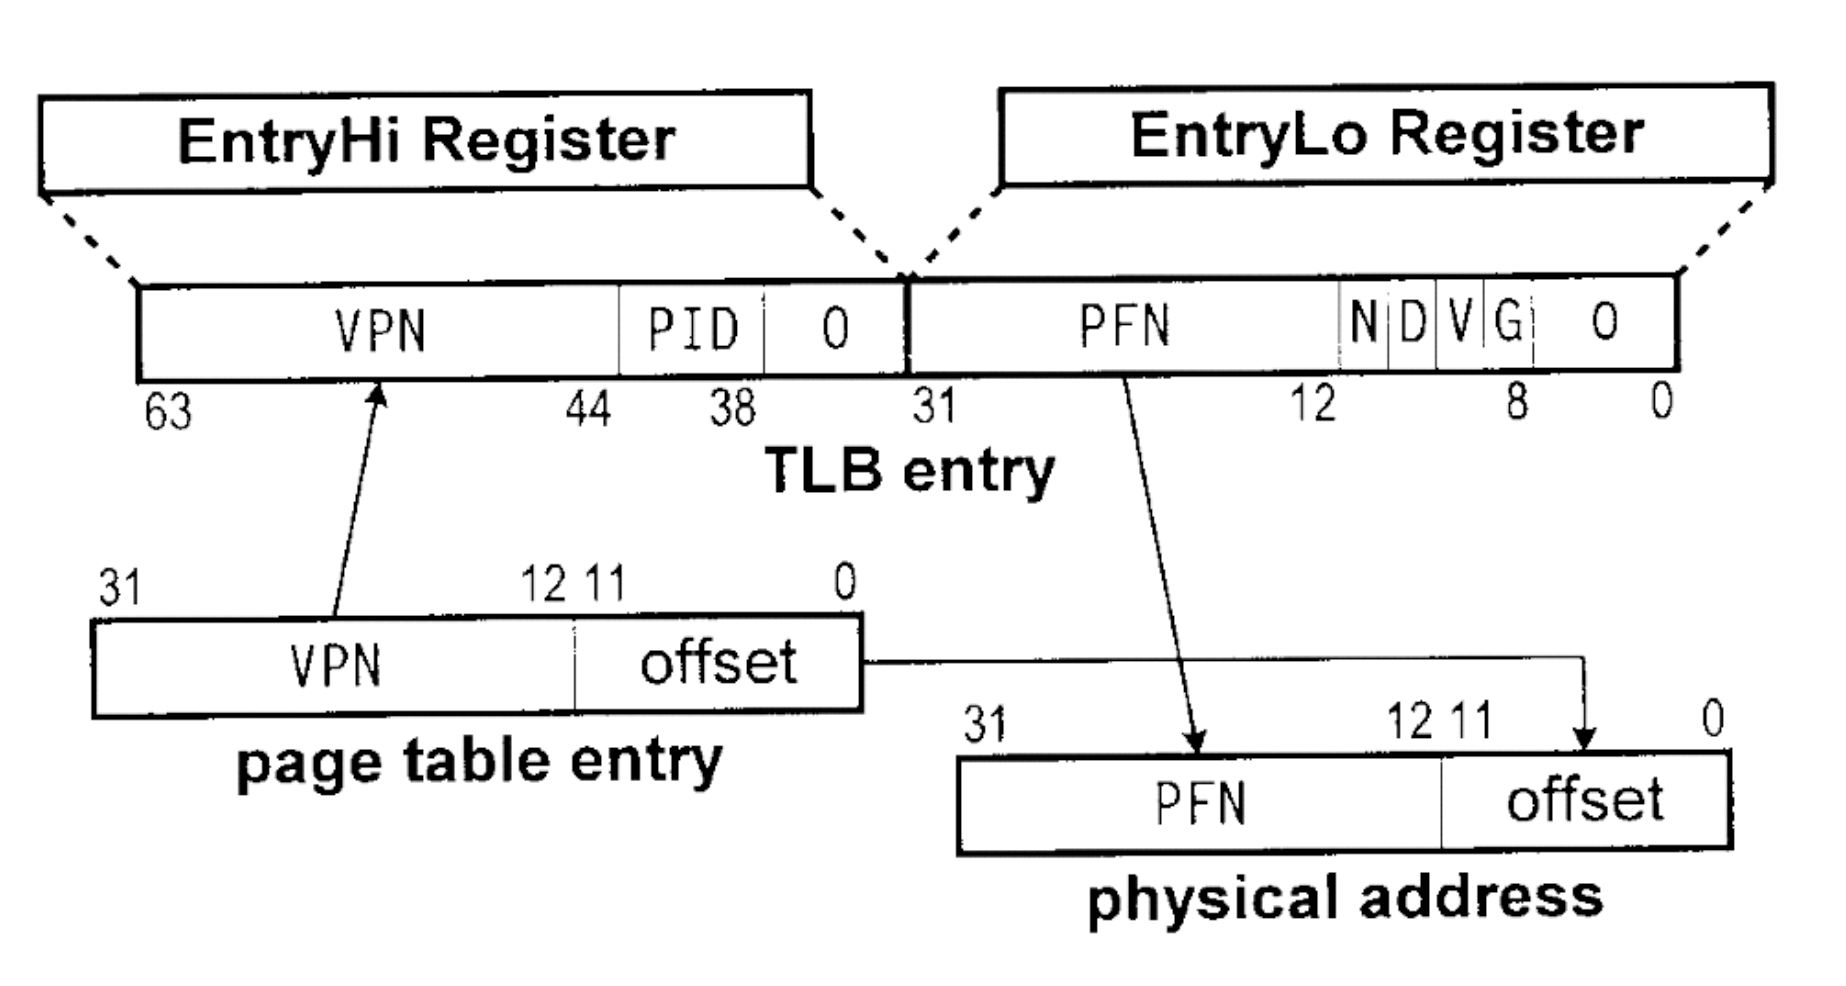
\includegraphics[width=0.7\textwidth]{Memoria Virtuale/images/MIPS R3000 address translation.png}
    \caption{Traduzione degli indirizzi MIPS R3000}
    \label{mips_r3000}
\end{figure}
da notare che non sono presenti né un referenced bit né un modified bit.

Quando si vuole effettuare una taduzione di indirizzi il numero di pagina virtuale è comparatto ocon tutte le entries della tlb simultaneamente. Se viene trovato un mache e il bit G non è settato, il PID dela entry è confrontato con il tblpid corruente salvato nell'entryhi register. Se sono uguali (o se il bit G è settato) e il bit V è settato il campo PFN contiene il valido numero di frame fisico. Altrimenti viene scatenata una eccezione TLBmiss, mentre per le operazioni di scrittura (store) il bit D deve essere settato altrimenti viene scatenata una eccezione TLBmod.
Dal momento che l'hardware non offre ulteriori supporti (come per esempio supporto per una page table), le eccezioni devono essere gestite direttamente dal kernel. Inoltre, visto che non ci sono bit referenced o modified questo comporta un ulteriori sforzo da parte del kernel in quanto deve sapere quali sono le pagine che sono state modificate in quanto devono essere salvate prima di essere riutilizzate. Per rendere questo possibile rendendo tutte le pagine "pulite" protette dalla scrittura (annullando il bit D nelle loro TLB) così da scatenare un'eccezione forzata TLBmod prima di scrivervi.

Questa architettura porta ad un gran numero di page faults visto che ogni TLBmiss deve essere gestita dal software (in questo caso OS161) in quanto il bisogno di tracciare le modifiche delle pagine e dei riferimenti causano un aumento dei page faults. Tuttavia questo è bilanciato da diversi aspetti tra i quali il più importante è che il segmento kseg0 non è mappato in TLB. In quanto viene utilizzato per salvare testo statico e dati del kernel il che aumenta la velocità di esecuzione del codice di kernel in quanto non occorre effettuare address translation. Infine, riduce anche il contenuto della TLB in quanto è utilizzata solamente per gli indirizzi utente e per strutture allocate dinamicamente di dati di kernel.
\subsubsection{OS161 e TLB}
OS161 offre delle funzioni a basso livello per gestire la TLB tra le quali:
\begin{itemize}
    \item \lstinline{tlb_write()}: modifica una specifica entry della TLB
    \item \lstinline{tlb_random()}: modifica una entry casuale della TLB
    \item \lstinline{tlb_read()}: legge una specifica entry della TLB
    \item \lstinline{tlb_probe()}: cerca uno specifico numero di pagina nella TLB
    \item \lstinline{tlb_reset()}: inizializza la TLB, è una funzione che viene invocata solamente all'avvio della sistema operativo infatti, a differenza delle altre funzioni che sono dichiarate in \lstinline{kern/arch/mips/include/tlb.h}, questa viene utilizzata solamente in \lstinline{start.S} che si trova in \lstinline{kern/arch/sys161/main}
\end{itemize}
Queste funzioni sono descritte nel file \lstinline{kern/arch/mips/vm/tlb-mips161.S} di seguito si mostra un piccolo snippet del codice:
\begin{lstlisting}[caption=Parte del file \lstinline{tlb-mips161.S} nella quale sono descritte le funzioni per gestire la TLB]
    /*. . .*/
    /*
    * tlb_write: use the "tlbwi" instruction to write a TLB entry
    * into a selected slot in the TLB.
    *
    * Pipeline hazard: must wait between setting entryhi/lo and
    * doing the tlbwi. Use two cycles; some processors may vary.
    */
   .text
   .globl tlb_write
   .type tlb_write,@function
   .ent tlb_write
tlb_write:
   mtc0 a0, c0_entryhi	/* store the passed entry into the */
   mtc0 a1, c0_entrylo	/*   tlb entry registers */
   sll  t0, a2, CIN_INDEXSHIFT  /* shift the passed index into place */
   mtc0 t0, c0_index	/* store the shifted index into the index register */
   ssnop		/* wait for pipeline hazard */
   ssnop
   tlbwi		/* do it */
   j ra
   nop
   .end tlb_write
   /*. . .*/
\end{lstlisting}

In questa parte di codice viene descritta una funzione assembly nella quale viene operata una scrittura nella TLB. Nello specifico:
\begin{enumerate}
    \item vengono scritti nella entry della TLB i valori salvati nei registri \lstinline{a0} e \lstinline{a1} rispettivamente nella \lstinline{c0_entryhi} e \lstinline{c0_entrylo}
    \item viene effettuato uno shift logico a sinistra di una quantità definita per trovare l'indice dello slot della TLB nella quale verrà scritto il contenuto
    \item viene salvato nel registro di controllo, questa operazione serve per determinare quale slot sarà sovrascritto
    \item le \lstinline{ssnop} sono delle operazioni di sicurezza (superscalar nope) per assicurarsi non avvengano dei pipeline hazards
    \item l'istruzione \lstinline{tlbwi} scrive effettivamente il contenuto nella TLB
\end{enumerate}
Anche le altre funzioni rimanenti sono dello stesso tipo, tutte di basso livello che lavorano con i registri di controllo e le entries della TLB.

\subsection{Memoria Virtuale in xv6}
\subsubsection{Introduzione}
Xv6 è basato sull'architettura RISC-V la quale ha istruzioni (sia kernel sia utente) che utilizzano indirizzi virtuali per essere mappati alla memoria RAM che prevede indirizzi fisici.

Xv6, in particolare, viene eseguito su Sv39 RISC-V che prevede che dei 64-bit a disposizione solamente i 39-bit inferiori vengono utilizzati, i restanti 25 superiori rimangono inutilizzati. Nella configurazione Sv39 una page table è un array di \(2^{27}\) page table entries (PTEs). Ogni entry contiene 44-bit nei quali viene scritto il numero di pagina, mentre nei restanti 10 dei flags.
\begin{figure}[hbt!]
    \centering
    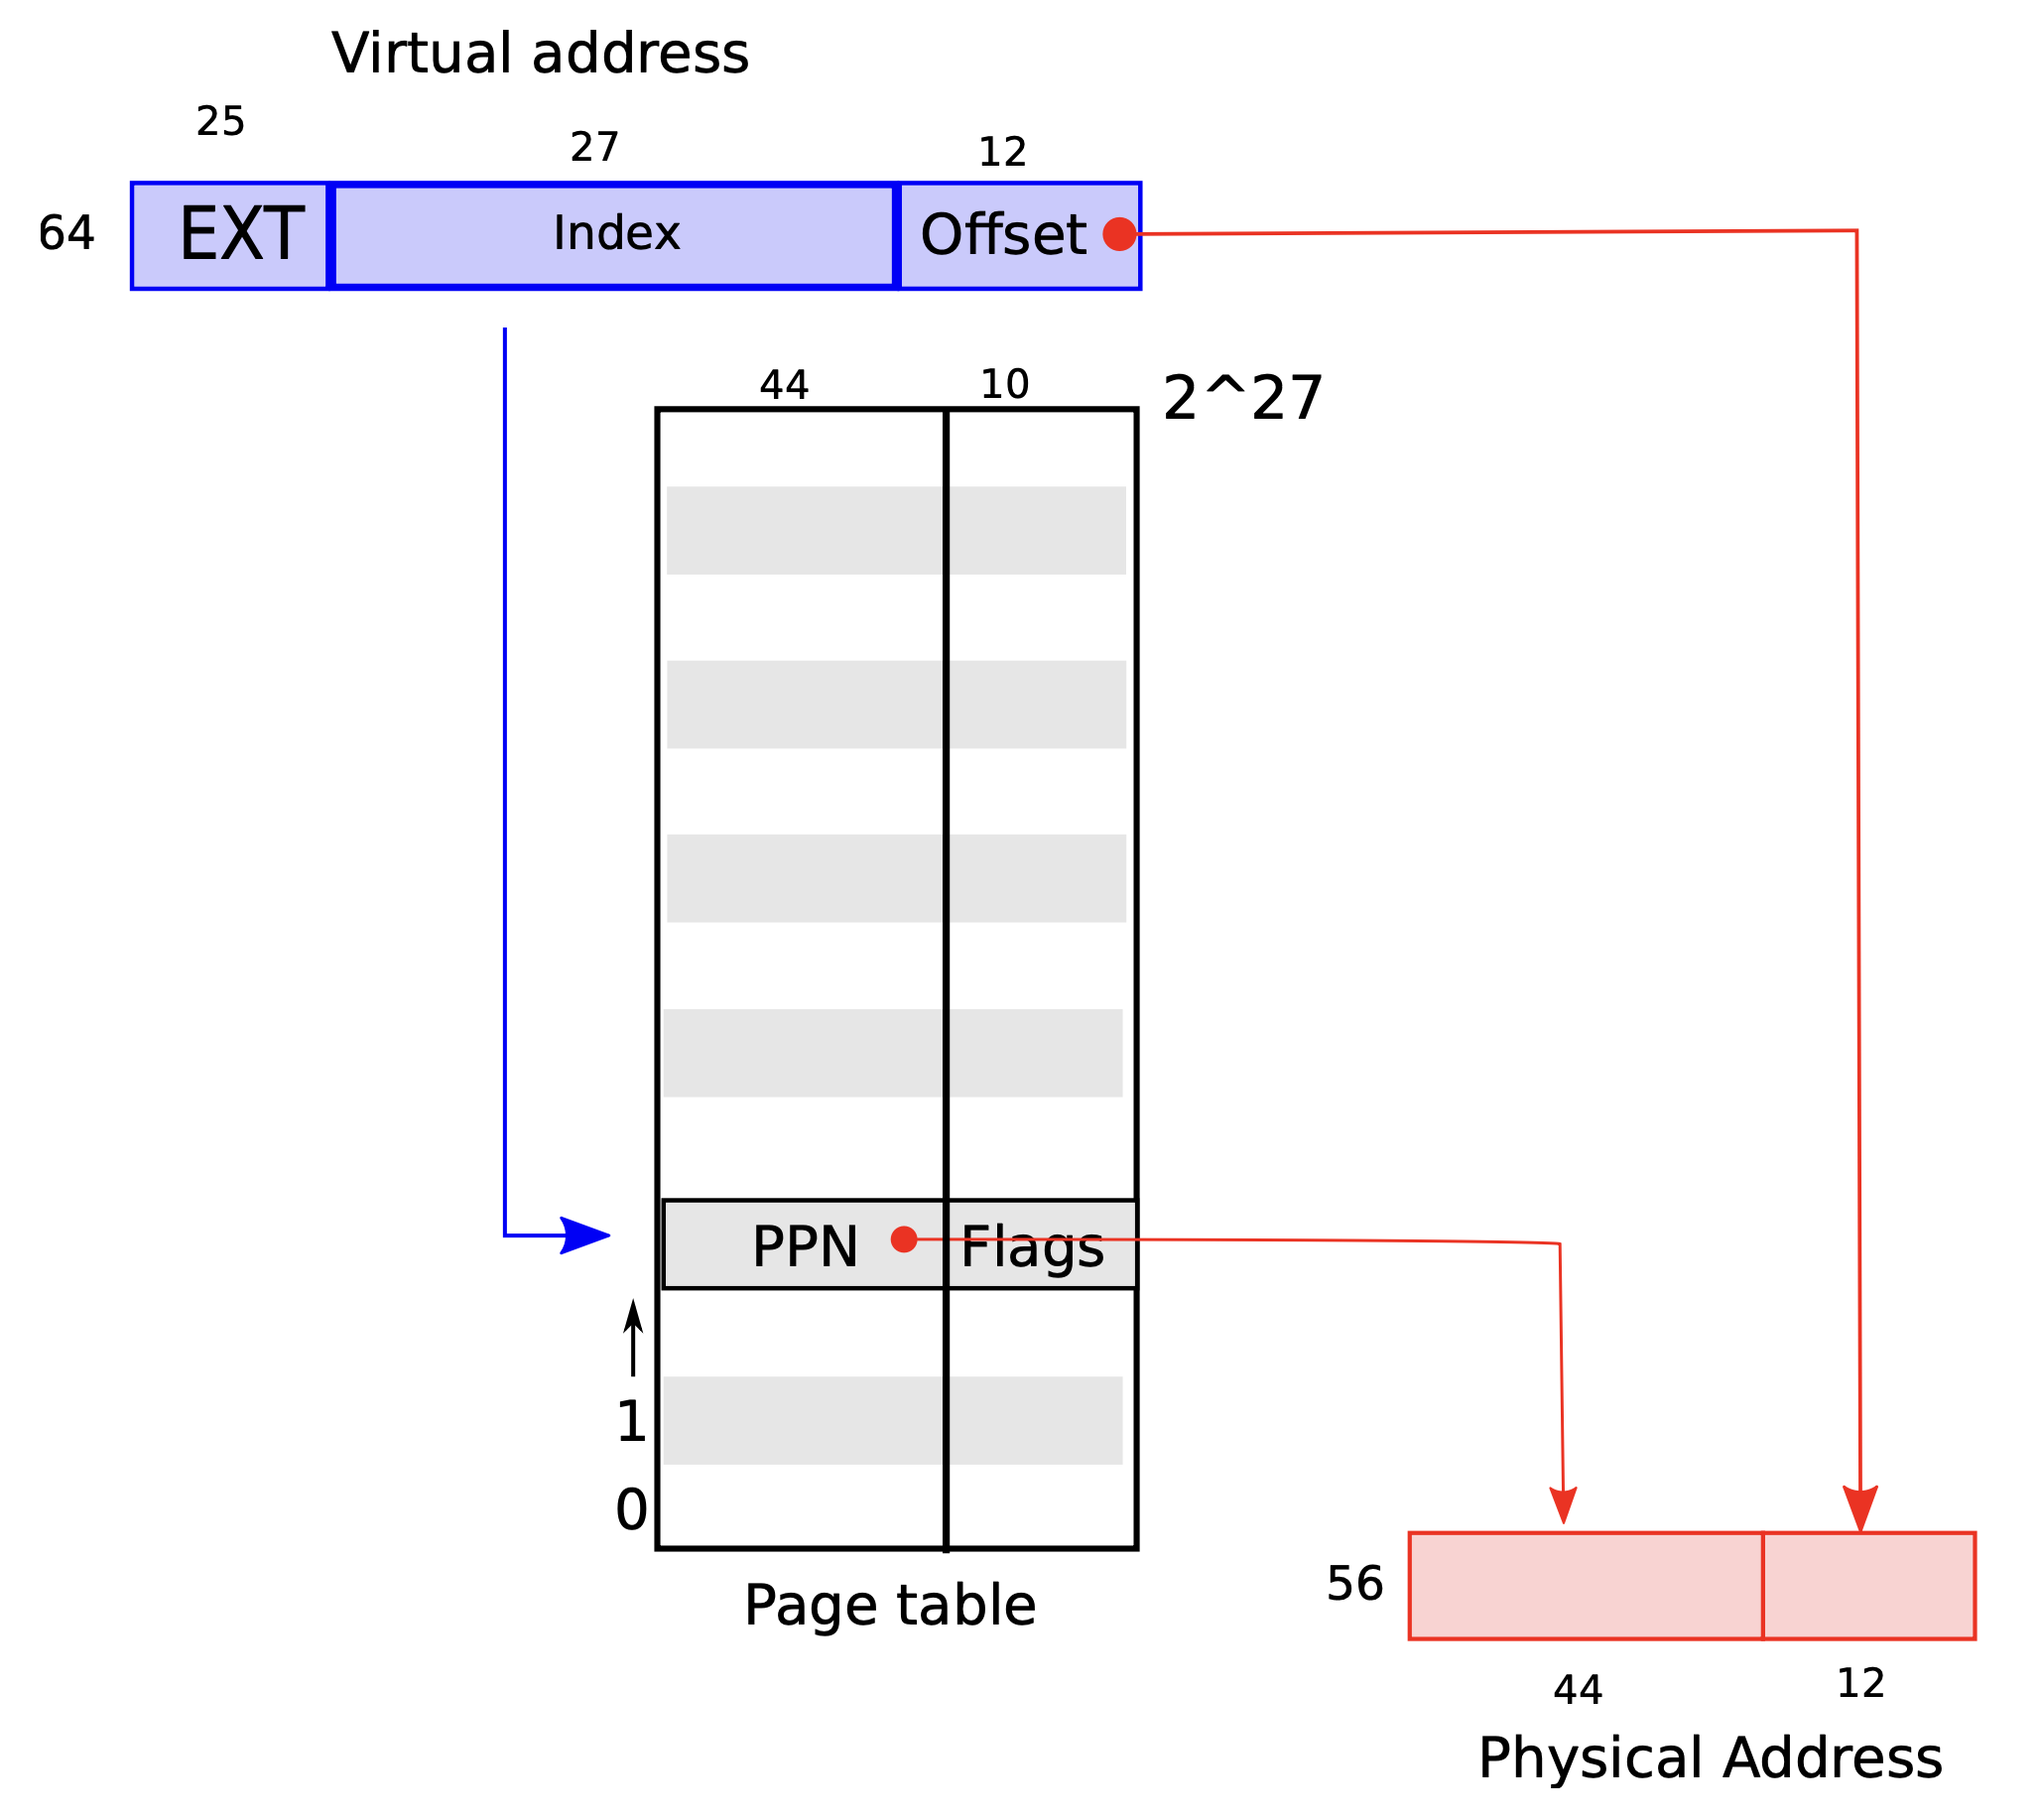
\includegraphics[width=0.5\textwidth]{Memoria Virtuale/images/virtual memory xv6.png}
    \caption{Rappresentazione degli indirizzi virtuali e fisici di Sv39 RISC-V}
    \label{fgi:xv6_mem}
\end{figure}

Come possiamo vedere dalla figura, dei 64 bit logici ne vengono utilizzati solamente 39, suddivisi in 27 in indice (in realtà indici come vedremo nella sezione successiva) della page table e 12 in offset di pagina, quindi ogni pagina misura \lstinline{4096 byte}. Tramite l'indice si trova il numero di pagina fisico (PPN) all'entry corrispondente nella page table che verrà utilizzato insieme all'offset per la scrittura dell'indirizzo fisico.

Il motivo per il quale è stata scelta la configurazione a 39 bit è giustificato dal fatto che un relativo spazio di indirizzamento virtuale, quindi al quale ogni processo può accedere, è di \lstinline{512 GB} il che, per gli sviluppatori è stato ritenuto opportuno.
\subsubsection{Traduzione degli indirizzi in Sv39 RISC-V}
Una CPU RISC-V traduce gli indirizzi virtuali in tre fasi. In memoria fisica vinee salvato un direttorio a tre livelli, la radice è una page table a 4096 byte che contiene 512 entries che contengono l'indirizzo fisico del prossimo nodo il quale, a sua volta è una page table di 512 entries che puntano all'ultima page table.
\begin{figure}[hbt!]
    \centering
    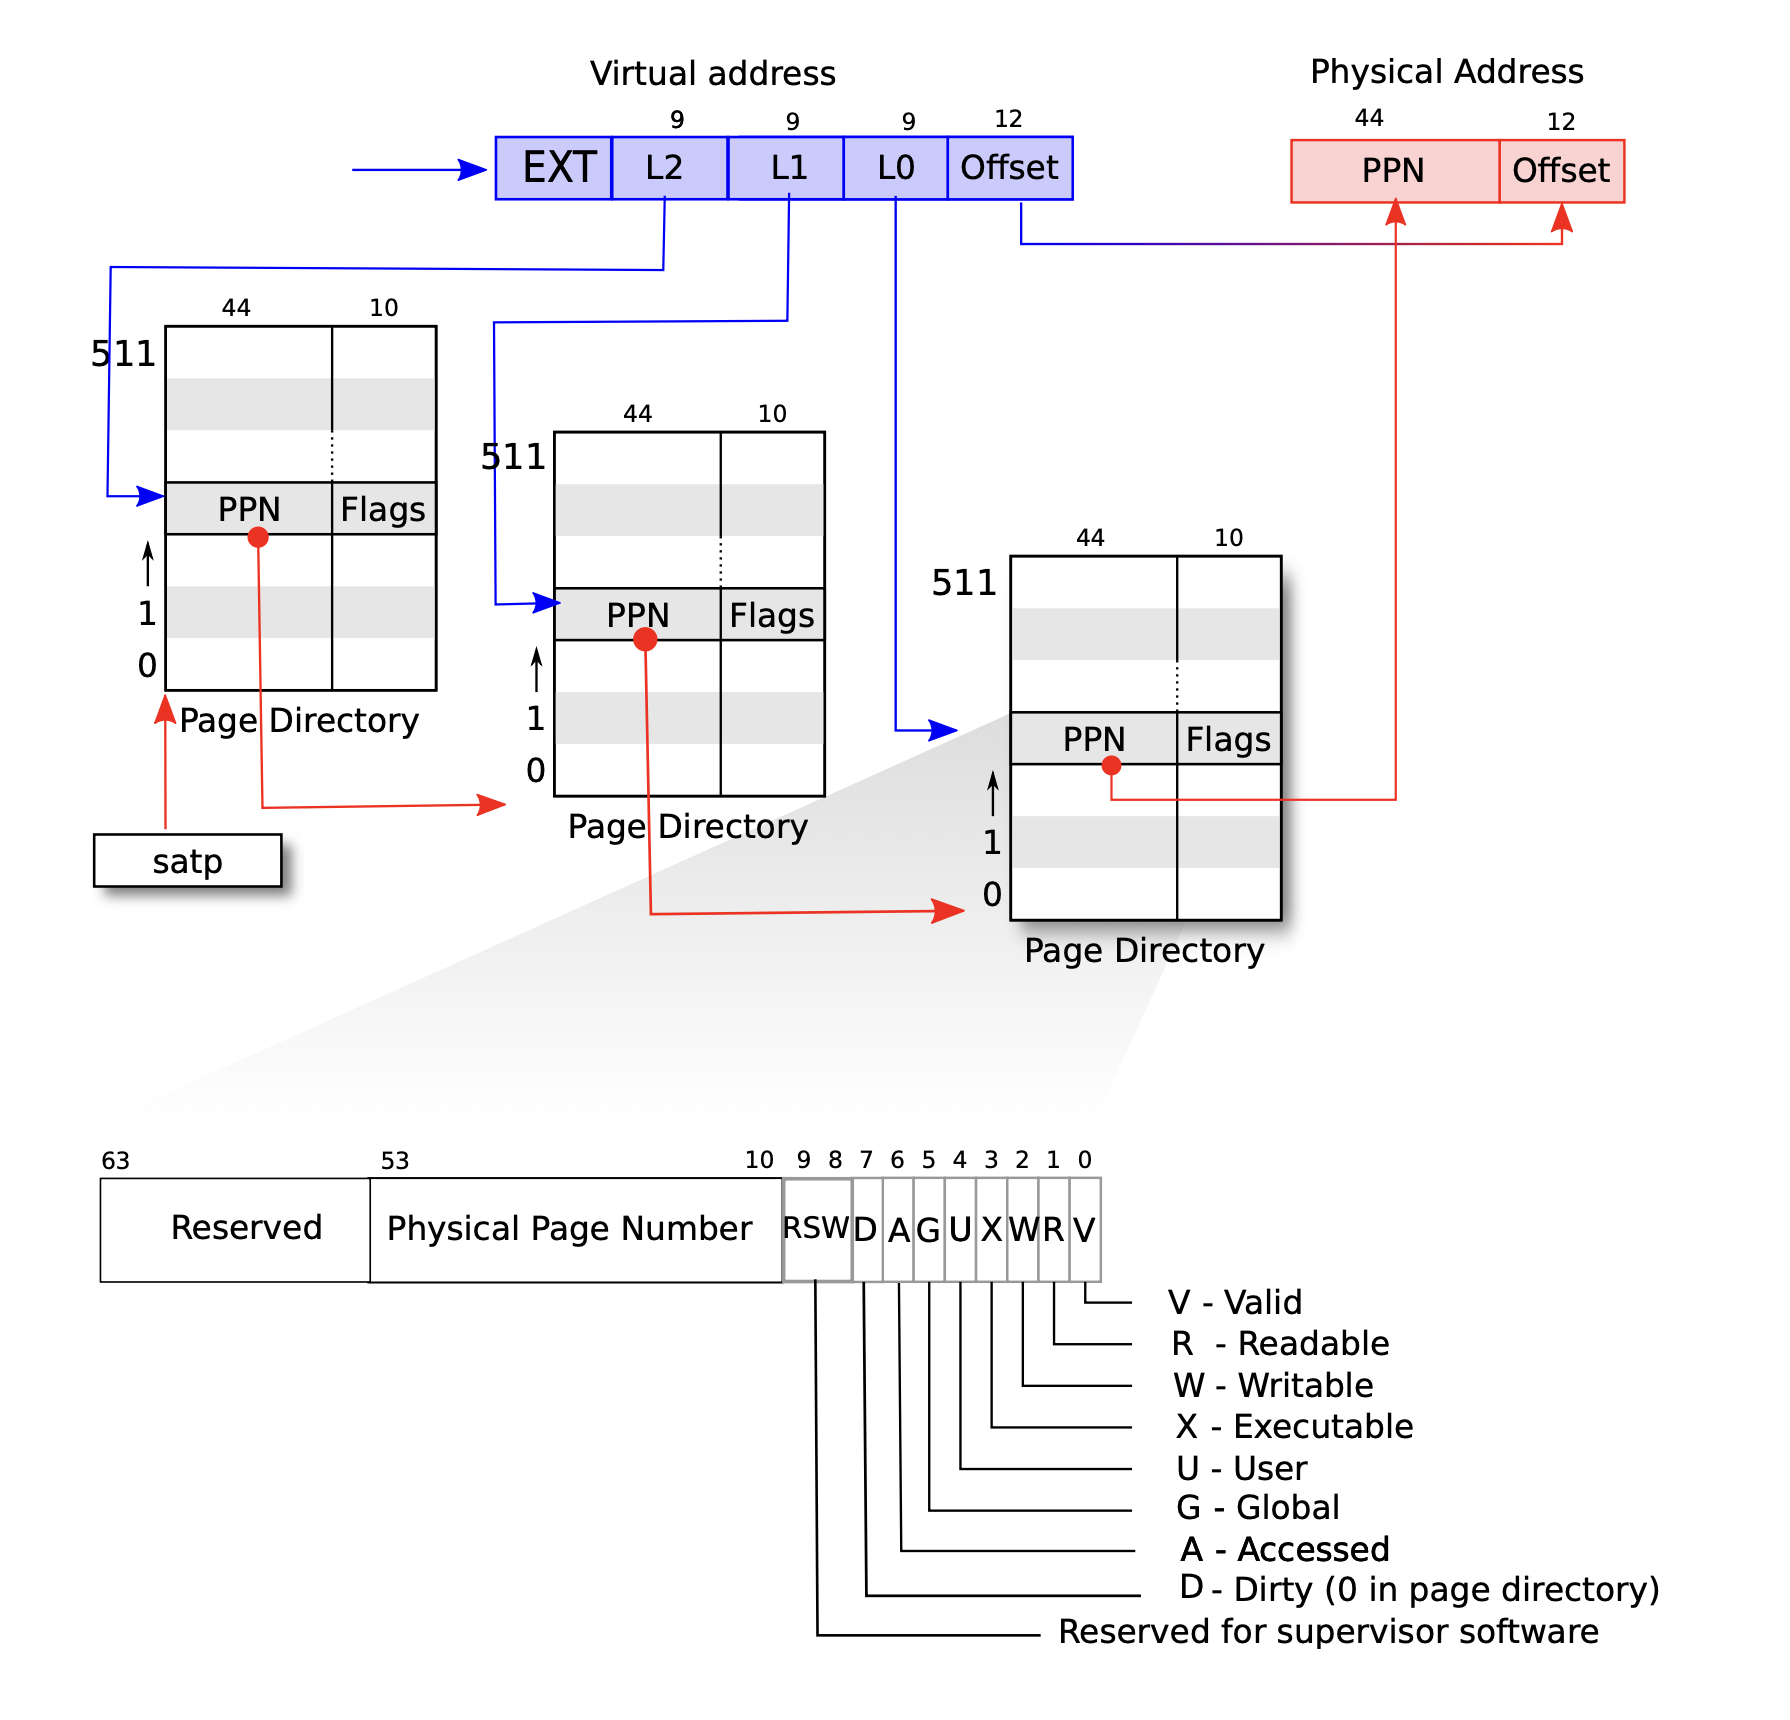
\includegraphics[width=\textwidth]{Memoria Virtuale/images/three-level paging.png}
    \caption{Dettagli della traduzione di Sv39 RISC-V}
    \label{fig:3-level_paging}
\end{figure}

Per quanto riguarda i flags sono numerosi e rappresentano:
\begin{itemize}
    \item RSW: riservato per i software superuser e può essere ignorato
    \item D: dirty flag indica se la pagina è stata modificata dall'ultima volta che il bit è stato pulito
    \item A: indica se è stato effettuato un qualsiasi tipo di accesso (lettura, scrittura o esecuzione) alla pagina dall'ultima volta che il bit è stato pulito 
    \item G: indica un global mapping ovvero un mapping che esiste in tutti gli spazi di indirizzamento (previene che la TLB possa essere liberata tramite la funzione \lstinline{LFENCE.VMA})
    \item U: indica se si può accedere alla pagina in user-level
    \item X, W, R: indicano se la pagina può essere eseguita, scritta o letta
    \item V: indica se la pagina è valida
\end{itemize}

\subsection{MMU in xv6}
\subsubsection{Il registro \lstinline{satp}}
Tutte le traduzioni eseguite dalla MMU cominciano dal \lstinline{satp} ovvero il registro Supervisor Address Translation and Protection. Leggendo il valore presente in questo registro si accede all'indirizzo fisico della root page table, in xv6 si può eseguire la seguente operazione grazie alla funzione \lstinline{r_satp()} che opera a basso livello chiamando una funzione assembler.
\begin{lstlisting}[caption=Funzione per leggere il valore del \lstinline{satp} presente in \lstinline{kernel/riscv.h}]
static inline uint64
r_satp()
{
  uint64 x;
  asm volatile("csrr %0, satp" : "=r" (x) );
  return x;
}
\end{lstlisting}

Questo registro è composto da tre parti che sono rispettivamente:
\begin{enumerate}
    \item MODE: indica la modalità di traduzione degli indirizzi adottata (in quanto Sv39 non è l'unica configurazione di RV64, in questo campo il valore 8 rappresenta proprio la configurazione adottata da xv6)
    \item ASID: address space identifier 
    \item PPN: indica il numero di pagina fisico, tuttavia è stato shifato a destra di 12 posizioni per essere salvato, quindi per accedere all'indirizzo originale si deve effettuare \lstinline{PPN<<12}
\end{enumerate}
\begin{figure}[hbt!]
    \centering
    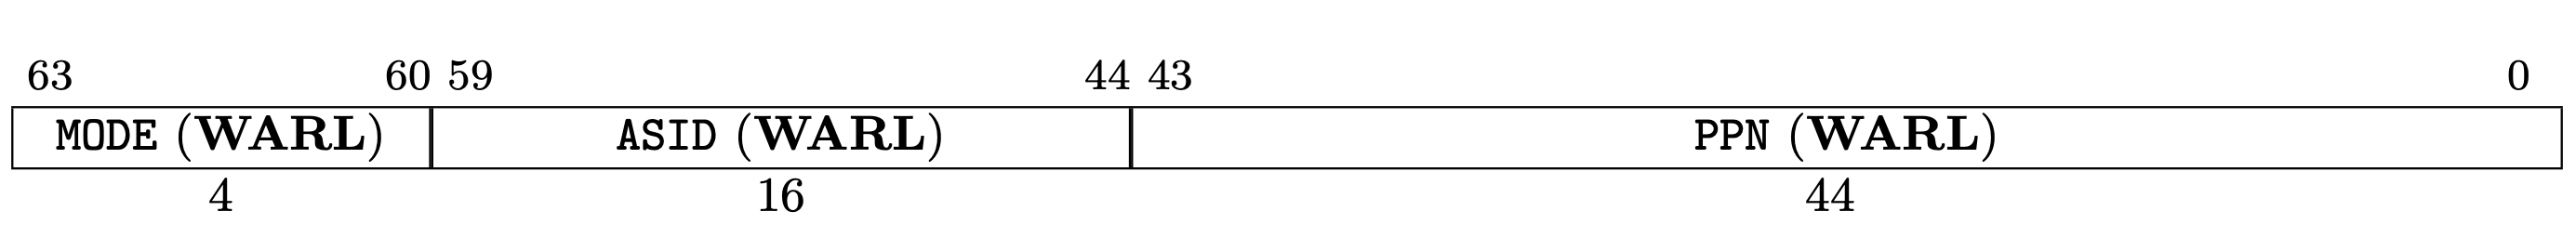
\includegraphics[width=\textwidth]{Memoria Virtuale/images/satp.png}
    \caption{La rappresentazione del \lstinline{satp} per la configurazione Sv39, con la suddivisione dei campi WARL (\textit{write any value, read legal value})}
    \label{fig:satp_sv39}
\end{figure}

\subsubsection{Traduzione degli indirizzi}
La MMU effettua la traduzione degli indirizzi seguendo i seguenti passaggi:
\begin{enumerate}
    \item legge il registro \lstinline{satp} e trova la root della page table in PPN calcolando, come detto in precedenza, l'indirizzo originale
    \item
\end{enumerate}
\section{Algoritmi di Scheduling}
\subsection{Introduzione}
\subsubsection{Obiettivi dello scheduling}
Un sistema operativo deve gestire molti processi contemporaneamente, ma la CPU può eseguirne solamente uno alla volta. Introduciamo quindi il concetto di scheduling il quale consiste nel decidere quale processo deve essere eseguito in un dato istante. Lo scheduling ha come obiettivo, quindi, quello di ottimizzare l'utilizzo della CPU trovando un bilanciamento tra:
\begin{itemize}
    \item massimizare il throughput: quanti processi sono eseguiti
    \item minimizzare la latenza: quanto tempo un processo aspetta per essere eseguito
    \item starvation: evitare che un processo non venga mai eseguito
    \item completare una processo entro un tempo predefinito
    \item massimizzare la percentuale di utilizzo del processore
\end{itemize}
\subsubsection{Preemption}
Introduciamo, inoltre, il concetto di preemption il quale indica se un algoritmo di scheduling e/o un processo è interrompibile o meno. Ci sono due possibilità inerenti al preemption:
\begin{itemize}
    \item la politica preemptive: 
    \begin{enumerate}
        \item un processo può essere interrotto per farne eseguire un altro, di conseguenza un processo non deve aspettare la terminazione di quello corrente prima di essere eseguito
        \item i processi interrotti aspettano che vengano eseguiti in memoria
        \item in ambienti multiprocessore un processo può essere rimosso dalla CPU alla quale è stato assegnato per effettuare un load balancing
        \item ha un costo maggiore in quanto la CPU deve tenere traccia dei processi in attesa, quindi salvare gli stati dei processi al tempo della interruzione, e avere un meccanismo che possa cambiare tra un processo all'altro
    \end{enumerate}

    \item la politica nonpreemptive:
    \begin{enumerate}
        \item un processo viene eseguito dall'inizio alla fine senza cedere il controllo della CPU a prescindere dalla durata o dalla priorità di altri processi in arrivo
        \item è rischioso in quanto un processo potrebbe bloccarne un altro per un tempo indefinito
        \item ha un costo minore in quanto non bisogna tenere traccia degli stati correnti dei processi in attesa e non c'è un sovraccarico della CPU con il cambio di processo
    \end{enumerate}
\end{itemize}

\subsubsection{Politiche degli algoritmi di scheduling}
Lo scheduling, quindi, è effettuato da un componente chiamato scheduler che, decide l'ordine temporale per il quale i processi devono accedere alla CPU. Esistono vari modi per scegliere l'ordine temporale e questo dipende da diversi fattori quali:
\begin{enumerate}
    \item la priorità del processo
    \item l'arrivo temporale della richiesta del processo
    \item la durata del processo
    \item il tempo di attesa in coda
\end{enumerate}
Le politiche di scheduling sono innumerevoli, ma tutti hanno come unico obiettivo quello di ottimizzare il rendimento della CPU. In particolare sono comuni a tutti gli algoritmi di scheduling l'equità, la scalabilità e la predicibilità, ovvero tutti i processi con le stesse caratteristiche sono tratti in maniera uguale che non varia dal numero dei processi da schedulare e, sapendo la politica adottata, si può risalire al risultato finale. Infine, in base a quali sono le caratteristiche che si vogliono rispettare, l'algoritmo di scheduling può essere più o meno complesso.
\subsection{Algoritmi di Scheduling in OS161}
Lo scheduler della versione base di OS161 offre un algoritmo di Round Robin con politica preemptive. Prima di esaminare in dettaglio il codice del sistema operativo spieghiamo brevemente il funzionamento dell'algoritmo in questione.
\subsubsection{Algoritmo di Round Robin}
Lo scheduling Round Robin è un algoritmo che si basa sulla divisione della durata dei processi in piccole porzioni chiamate quanta (il plurale di quantum) che vengono eseguite ciclicamente in base all'ordine di arrivo e senza concetto di priorità.
\begin{figure}[hbt!]
    \centering
    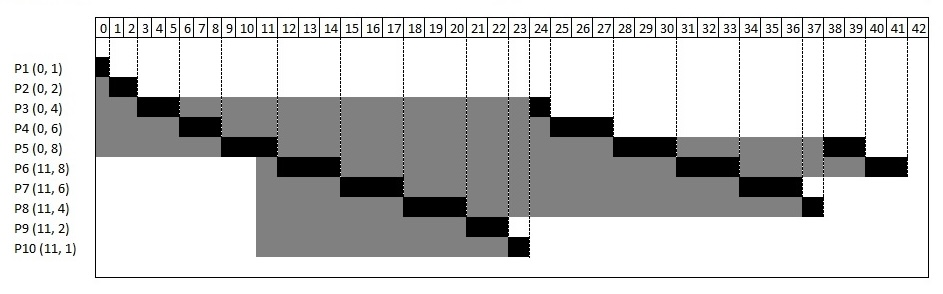
\includegraphics[width=\textwidth]{Algoritmi di Scheduling/images/round_robin.jpg}
    \caption{Rappresentazione temporale di uno scheduling round robin. In questo esempio i processi sono descritti da una coppia di valori che rappresentano il tempo di arrivo e la durata. Il time quantum è di 3 unità temporali e l'area grigia rappresenta il tempo di attesa di un processo prima di essere stato eseguito completamente.}
    \label{round_robin}
\end{figure}

Come possiamo notare dalla figura, è uno scheduling di tipo preemptive in quanto ogni quantum di tempo passato, se il processo in corso non è terminato viene sospeso e si passa al successivo. I processi aspettano in una coda ordinata in base al tempo di arrivo, i processi che devono essere eseguiti vengono estratti da questa coda e vengono eliminati da essa solamente una volta terminati completamente. Infine, è anche starvation free in quanto tutti i processi hanno la stessa priorità e possibilità di essere eseguiti a prescindere dalla durata di essi.

\subsubsection{Scheduler in OS161}
Una volta esaminato il comportamento ad alto livello dello scheduler, passiamo a studiare il funzionamento a basso livello.

I principali dettagli implementativi dell'algoritmo sono descritti in \lstinline{kern/thread/clock.c} in cui troviamo la definizione temporale
\begin{lstlisting}[caption={Vincoli temporali in \lstinline{clock.c}}]
#define SCHEDULE_HARDCLOCKS	4
#define MIGRATE_HARDCLOCKS	16
\end{lstlisting}
che rappresentano rispettivamente ogni quanti cicli di clock hardware avviene lo scheduling e la migrazione (in caso di architettura multiprocessore si può spostare il thread in un'altra CPU se sono libere o meno occupate).

Lo scheduling è gestita dalla funzione \lstinline{hardclock()} che si trova in \lstinline{kern/thread/clock.c} che a sua volta chiama la funzione per schedulare o per migrare il thread e viene chiamata un numero fisso \lstinline{HZ} di volte al secondo.
\begin{lstlisting}[caption=Quanti hardcloks al secondo in \lstinline{clock.h}]
#define HZ  100
\end{lstlisting}

Le funzioni che gestiscono lo scheduling e la migrazione del thread sono rispettivamente \lstinline{schedule()} e \lstinline{thread_consider_migration()}, in questa sezione ci concentreremo sulla prima.
La funzione che le racchiude viene chiamata (da ogni CPU) 100 volte al secondo e semplicemente incrementa il numero di cicli di clock e se è un multiplo di \lstinline{MIGRATE_HARDCLOCKS} chiama la funzione dedicata alla migrazione mentre se è multiplo di \lstinline{SCHEDULE_HARCLOCKS} viene chiamata la funzione per lo scheduling. Essa nella versione base di OS161 è vuota in quanto non è previsto nessuna forma articolata di scheduling, ma qualora si volesse implementare la si dovrebbe modificare presente in \lstinline{kern/thread/thread.c}

\begin{lstlisting}[caption={\lstinline{hardclock()} in \lstinline{clock.c}}]
void
hardclock(void)
{
	curcpu->c_hardclocks++;
	if ((curcpu->c_hardclocks % MIGRATE_HARDCLOCKS) == 0) {
		thread_consider_migration();
	}
	if ((curcpu->c_hardclocks % SCHEDULE_HARDCLOCKS) == 0) {
		schedule();
	}
	thread_yield();
}
\end{lstlisting}

L'unico scheduling effettuato dal sistema operativo è eseguito dalla funzione \lstinline{thread_yield()} che a sua volta chiama \lstinline{thread_switch(S_READY,NULL,NULL)}. Essa ha come parametro fondamentale \lstinline{S_READY} che rappresenta lo stato del thread, quindi è pronto per essere eseguito che all'interno di uno switch case, indirizzerà il thread corrente all'interno della funzione \lstinline{thread_make_runnable}.

\begin{lstlisting}[caption={La funzione \lstinline{thread_make_runnable} in \lstinline{kern/thread/thread.c}}]
static
void
thread_make_runnable(struct thread *target, bool already_have_lock)
{
	struct cpu *targetcpu;

	/* Lock the run queue of the target thread's cpu. */
	targetcpu = target->t_cpu;

	if (already_have_lock) {
		/* The target thread's cpu should be already locked. */
		KASSERT(spinlock_do_i_hold(&targetcpu->c_runqueue_lock));
	}
	else {
		spinlock_acquire(&targetcpu->c_runqueue_lock);
	}

	/* Target thread is now ready to run; put it on the run queue. */
	target->t_state = S_READY;
	threadlist_addtail(&targetcpu->c_runqueue, target);

	if (targetcpu->c_isidle && targetcpu != curcpu->c_self) {
		/*
		 * Other processor is idle; send interrupt to make
		 * sure it unidles.
		 */
		ipi_send(targetcpu, IPI_UNIDLE);
	}

	if (!already_have_lock) {
		spinlock_release(&targetcpu->c_runqueue_lock);
	}
}
\end{lstlisting}

Questa funzione semplicemente inserisce il thread nella coda dei thread in esecuzione. Come possiamo vedere nel file \lstinline{kern/include/thread_list.h} nella versione base di OS161 la coda è semplicemente una lista doppio puntata. Quindi qualora si volesse implementare un algoritmo più sofisticato all'interno del sistema operativo si dovrebbe modificare la funzione \lstinline{schedule()}, citata sopra, accedendo alla coda dei thread e modificando il loro ordine per decidere lo scheduling.

\begin{lstlisting}[caption={Struttura dati della coda dei thread in esecuzione}]
struct threadlistnode {
 struct threadlistnode *tln_prev;
 struct threadlistnode *tln_next;
 struct thread *tln_self;
};

struct threadlist {
	struct threadlistnode tl_head;
	struct threadlistnode tl_tail;
	unsigned tl_count;
};
\end{lstlisting}

\subsection{Algoritmi di Scheduling in xv6}

\end{document} 
